\documentclass[11pt, a4paper]{article}

%Preambuła dokumentu
\usepackage{graphicx}
\usepackage{rotating}
\usepackage{subfigure}
\usepackage{float}
\usepackage{epic}
\usepackage{psfrag}
\usepackage{epstopdf}
\usepackage{curves}
\usepackage{listings}
\usepackage{verbatim}
\usepackage{alltt}
\usepackage{fp}
\usepackage{calc}
\usepackage{ifthen}
\usepackage{amssymb}
\usepackage{amsmath}
\usepackage[polish]{babel}
\usepackage{polski}
\usepackage{geometry}
\usepackage{array}
\usepackage{multirow}
\usepackage{enumerate}
\usepackage{enumitem}
\usepackage[ampersand]{easylist}
\usepackage{changepage}
\usepackage{hyperref}
\usepackage{url}
%\usepackage{parskip}
%\setlength{\parskip}{1ex}
\usepackage[OT4]{fontenc}
\usepackage[utf8]{inputenc}
\usepackage{color}
\definecolor{bluekeywords}{rgb}{0.13,0.13,1}
\definecolor{greencomments}{rgb}{0,0.5,0}
\definecolor{redstrings}{rgb}{0.9,0,0}

% Koniec preambuły dokumentu

% Tekst dokumentu
\begin{document}
\begin{titlepage}

\newcommand{\HRule}{\rule{\linewidth}{0.5mm}} % Defines a new command for the horizontal lines, change thickness here

\center % Center everything on the page

%----------------------------------------------------------------------------------------
%	HEADING SECTIONS
%----------------------------------------------------------------------------------------

\textsc{\LARGE Politechnika Wrocławska\\}
\vspace{0.5cm}
\textsc{\large Automatyka i Robotyka, ARR, W4}\\[4.5cm] % Name of your university/college

\textsc{\Large Wizualizacja Danych Sensorycznych}\\[0.5cm] % Major heading such as course name
\textsc{\large Sprawozdanie Okresowe Nr 2/3 \\ - Rezultaty prawie końcowe -}\\[0.5cm] % Minor heading such as course title

%----------------------------------------------------------------------------------------
%	TITLE SECTION
%----------------------------------------------------------------------------------------

\HRule \\[0.6cm]
{ \huge \bfseries Wizualizacja rozkładu ciśnienia cieczy na podstawie symulacji komputerowej}\\[0.6cm] % Title of your document
\HRule \\[3.5cm]

%----------------------------------------------------------------------------------------
%	AUTHOR SECTION
%----------------------------------------------------------------------------------------

\begin{minipage}{0.4\textwidth}
\begin{flushleft} \large
\emph{Autorzy:}\\
\textsc{Balawender} Adam % Your name
\end{flushleft}
\end{minipage}
~
\begin{minipage}{0.4\textwidth}
\begin{flushright} \large
\emph{Prowadzący:} \\
Dr inż. Bogdan \textsc{Kreczmer} % Supervisor's Name
\end{flushright}
\end{minipage}\\[0.1cm]

\begin{minipage}{0.4\textwidth}
\begin{flushleft} \large
\textsc{Kwieciński} Krzysztof \\
\end{flushleft}
\end{minipage}
~
\begin{minipage}{0.4\textwidth}
\begin{flushright} \large
\end{flushright}
\end{minipage}%\\[4cm]

\vfill

% If you don't want a supervisor, uncomment the two lines below and remove the section above
%\Large \emph{Author:}\\
%John \textsc{Smith}\\[3cm] % Your name

%----------------------------------------------------------------------------------------
%	DATE SECTION
%----------------------------------------------------------------------------------------

{\large \today}%\\[3cm] % Date, change the \today to a set date if you want to be precise

%----------------------------------------------------------------------------------------
%	LOGO SECTION
%----------------------------------------------------------------------------------------

%\includegraphics{Logo}\\[1cm] % Include a department/university logo - this will require the graphicx package

%----------------------------------------------------------------------------------------

%\vfill % Fill the rest of the page with whitespace

\end{titlepage}

\tableofcontents
\clearpage
\pagenumbering{arabic}% Arabic page numbers (and reset to 1)
% opis rozwiazywanego problemu  

\section{Opis projektu}
Zgodnie z tematem projektu zajmiemy się komputerową symulacją zachowania cieczy oraz wizualizacją jej stanu i~rozkładu ciśnienia w zbiorniku z płynem.

Symulacja będzie obejmowała ruch cieczy w przekroju 2D wybranego naczynia. Ciecz zostanie przedstawiona na płaszczyźnie jako zbiór oddziaływujących ze sobą cząsteczek.
Postaramy się, żeby jej zachowanie było możliwie zbliżone do rzeczywistego.
Ruch płynu zostanie zamodelowany metodą numeryczną SPH (\textit{smoothed particle hydrodynamics - wygładzona hydrodynamika cząstek}).
Pozwoli to na realistyczne odwzorowanie zachowania cieczy.
Możliwe będzie badanie cieczy o różnych parametrach, dlatego też modelowane będą jej właściwości fizyczne: gęstość i~lepkość.
Dodatkowo mierzone będzie ciśnienie cieczy i zostanie ono zwizualizowane jako odcień koloru płynu.
Im będzie on ciemniejszy, tym wyższe ciśnienie będzie odzwierciedlał.

Aplikacja zostanie napisana w języku \textsf{C++}, przy użyciu biblioteki \textsf{Qt}.
% zaktualizowany harmonogram wraz z wymienieniem tych elementow poprzedniego harmonogramu, ktore udalo sie zrealizowac

\section{Plan pracy}
\subsection{Podział obowiązków}
Projekt zakłada powiązanie symulacji numerycznej (back-end) z aplikacją prezentującą wyniki w~formie graficznej (front-end). Za pierwszą z ww. części odpowiedzialny będzie Adam
Balawender, za drugą Krzysztof Kwieciński. Obie części powinny mieć możliwość niezależnego uruchomienia, co ułatwi ich testowanie we wstępnych etapach oraz ocenę w końcowym etapie projektu.

\subsection{Harmonogram}
Termin rozpoczęcia projektu to 9.03.2015, natomiast termin zakończenia realizacji projektu przewidziany jest na 11.06.2015. Oznacza to, że okres prac nad projektem wynosi w przybliżeniu XIII tygodni.

Do tej pory udało się nam zrealizować zadania z tygodni I - X z założonego wcześniej harmonogramu, \cite{ABKKWstepne}. Na dzień dzisiejszy prace nad projektem trwają już przez dziesięć tygodni, zatem projekt wykonywany jest w terminie. 

Aktualny harmonogram przedstawiony znajduje się poniżej.

\renewcommand{\arraystretch}{1.8}
\begin{tabular}{l || c | c }
\hline
Tydzień & Adam & Krzysztof                                                                                                                            \\\hline \hline
    I    & \multicolumn{2}{ c }{ Opis projektu                                                                                                      } \\\hline
    II   & \multicolumn{2}{ c }{ Przegląd bibliotek Qt, szkic GUI                                                                                   } \\\hline
    III  & \multicolumn{2}{ c }{ Zapoznanie się z metodą SPH (Smoothed Particle Hydrodynamics)                                                      } \\\hline
    IV, V   & \multicolumn{2}{ c }{ Ustalenie struktur danych oraz API modułów                                                                         } \\\hline
    VI, VII    & \parbox[c]{6cm}{Implementacja klas zbiornika oraz cząsteczek cieczy }    & \parbox[c]{6cm}{Stworzenie statycznej wizualizacji zbiornika  } \\\hline
    VIII, IX   & \parbox[c]{6cm}{Dodanie wizualizacji położenia cząstek cieczy} & \parbox[c]{6cm}{Implementacja metod uaktualniania położenia cząsteczek} \\\hline
    X  & \multicolumn{2}{ c }{ Analiza błędów działania programu i skorygowanie ich                                                                 } \\\hline
    XI   & Wizualizacja ciśnienia w punktach     &   Wyznaczanie ciśnienia w punkach zbiornika                                                      \\\hline
    XII    & \multicolumn{2}{ c }{ Weryfikacja projektu z założeniami i odpowiednie modyfikacje programu                                                                                 } \\\hline
    XIII  & \multicolumn{2}{ c }{ Napisanie raportu końcowego                                                                                        } \\\hline
\end{tabular}

\subsection{Kamienie milowe}
\begin{enumerate}[label=K\arabic*{.}]
    \item Przeanalizowanie artykułów na temat SPH i zapoznanie się z tą metodą
    \item Zaimplementowanie struktur danych, modelu cieczy i relacji między cząsteczkami
    \item Wizualizacja symulowanego stanu cieczy
    \item Wizualizacja ciśnienia w poszczególnych punktach zbiornika
    \item Skończona dokumentacja
\end{enumerate}

\newpage
\subsection{Diagram Gantta}
\begin{figure}[H] 
 \begin{center}
  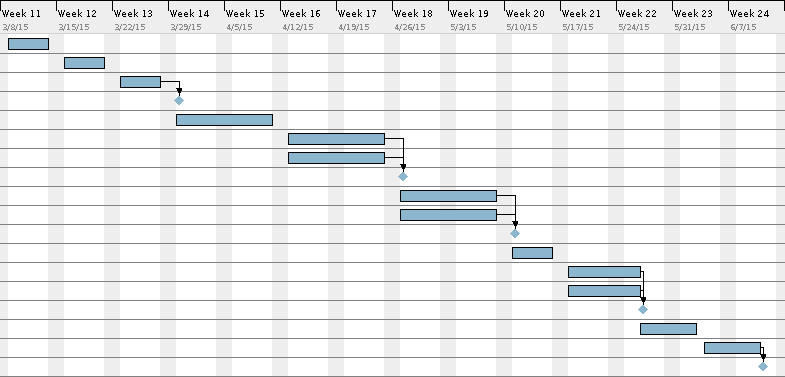
\includegraphics[width=\textwidth]{../harmonogram/gantt_uaktualniony.png}
 \end{center}
 \caption{Diagram Gantta}
 \label{fig:gantt}
\end{figure}
 

% opis funkcjonalnosci aplikacji

\section{Funkcjonalności aplikacji}
Najistotniejsze funkcjonalności aplikacji to:
\begin{itemize}
    \item symulacja zachowania modelu cieczy przy obracaniu zbiornikiem,
    \item możliwość wyzerowania pionowej składowej wektora grawitacji,
    \item programowa możliwość przedefiniowania parametrów cieczy (eg. gęstości, lepkości) oraz warunków początkowych,
    \item zmiana szybkości symulacji,
    \item możliwość obserwacji wyniku symulacji (położenia cząsteczek i~rozkładu ciśnień) oraz interakcji.
\end{itemize}

Aplikacja umożliwia zasymulowanie zachowania cieczy od zadanych warunków początkowych. Daje użytkownikowi możliwość interakcji - poruszania zbiornikiem za pomocą \textit{slidera}. Symulacja odzwierciedla zachowanie cząsteczek na Ziemi, a dzięki możliwości wyzerowania pionowej składowej wektora grawitacji, również w~Kosmosie i w warunkach mikrograwitacji. Programowo dostępna jest zmiana wszystkich założonych parametrów cząsteczki cieczy. Wybrano model wody uznając go za najbardziej intuicyjny i atrakcyjny wizualnie w symulacji. Podczas działania aplikacji w~jej okienku obserwować można komputerowo zamodelowany ruch płynu wraz z rozkładem panujących w~nim ciśnień. Symulacja może być zatrzymywana i ponownie uruchamiana, a jej szybkość zmieniana. Rysunek \ref{fig:gui} przedstawia przykładowy zrzut ekranu działającej aplikacji.

% opis interfejsu graficznego aplikacji

\section{Interfejs graficzny}
Wygląd interfejsu graficznego aplikacji przedstawiony jest na rysunku \ref{fig:gui}.

\begin{figure}
 \begin{center}
  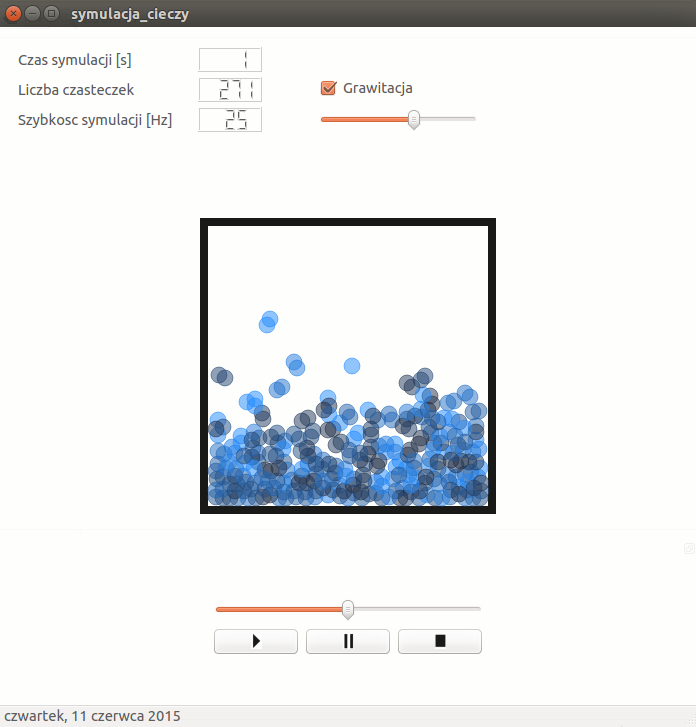
\includegraphics[width=\textwidth]{./rysunki/gui}
 \end{center}
 \caption{Interfejs graficzny aplikacji}
 \label{fig:gui}
\end{figure}
\begin{itemize}
    \item
W centralnej części aplikacji widoczny jest jej główny element, czyli zbiornik z~cząsteczkami. Pod nim znajduje się \textit{slider} pozwalający na przechylanie zbiornika.

    \item
Cząsteczki oraz okienko aplikacji są częściowo przezroczyste, co nadaje mu nowoczesny wygląd.

    \item
Użytkownik za pomocą trzech przycisków umiejscowionych na dole ekranu może sterować symulacją, a mianowicie ją: uruchomić, zamrozić lub zatrzymać.

    \item
W lewej górnej części okienka znajdują się elementy informacyjne pozwalające śledzić parametry symulacji: jej czas trwania, symulowaną liczbę cząsteczek oraz szybkość odświeżania wizualizacji. Na prawo od nich umiejscowione są elementy umożliwiające interakcję użytkownika z aplikacją: \textit{slider} pozwalający na zmianę szybkości symulacji oraz pole typu \textit{checkbox} zmieniające wektor grawitacji.

    \item
Na widocznej w dole ekranu belce statusowej wyświetlana jest aktualna data. W~pasku menu dostępna jest opcja zamknięcia aplikacji.

    \item
Rozkład elementów interfejsu graficznego jest odpowiednio modyfikowany przy zmianie wymiarów okienka.
\end{itemize}

\section{Diagram klas}
Założony diagram klas przedstawiony jest na rysunku \ref{fig:diagram_klas_gui}.

\begin{figure}[H]
 \begin{center}
  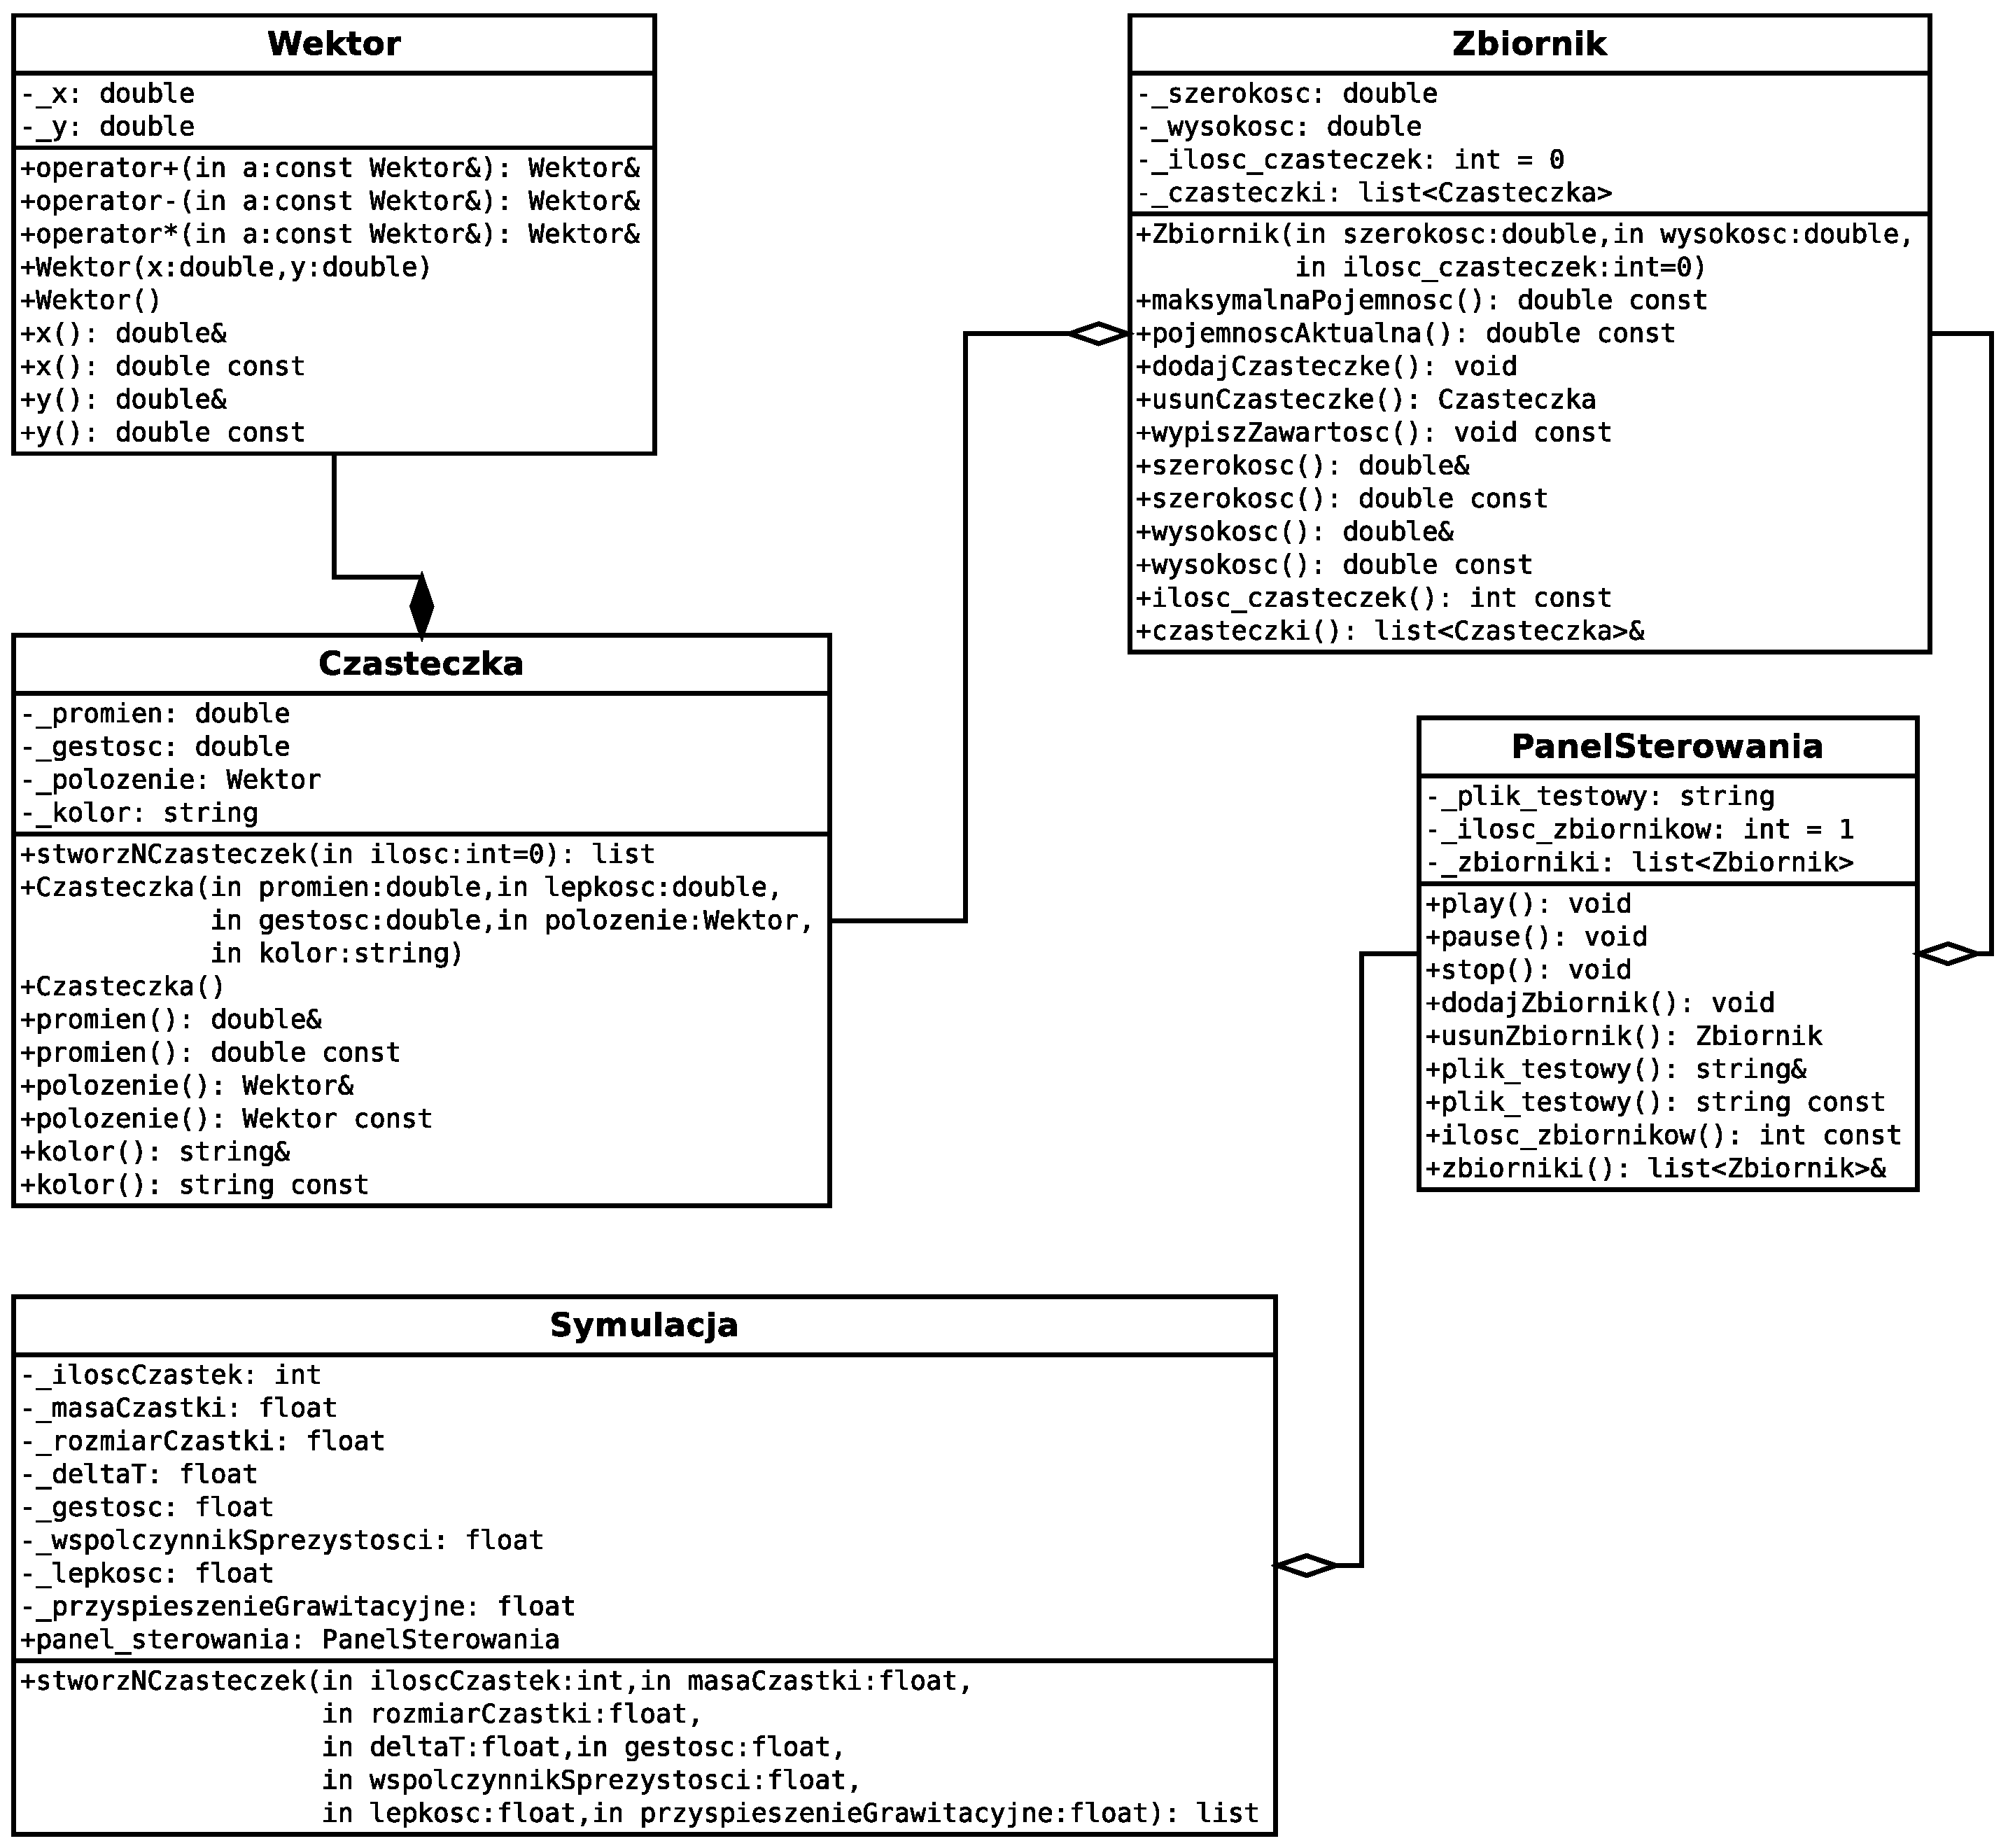
\includegraphics[width=\textwidth] {rysunki/diagram_klas3}
 \end{center}
 \caption{Diagram klas dla interfejsu graficznego}
 \label{fig:diagram_klas_gui}
\end{figure}

% diagram przeplywu sterowania lub schemat blokowy

\section{Przepływ sterowania}
Diagram przepływu sterowania przedstawiony jest na rysunku \ref{fig:diagram_przeplywu_gui}.

\begin{figure}[H]
 \begin{center} 
  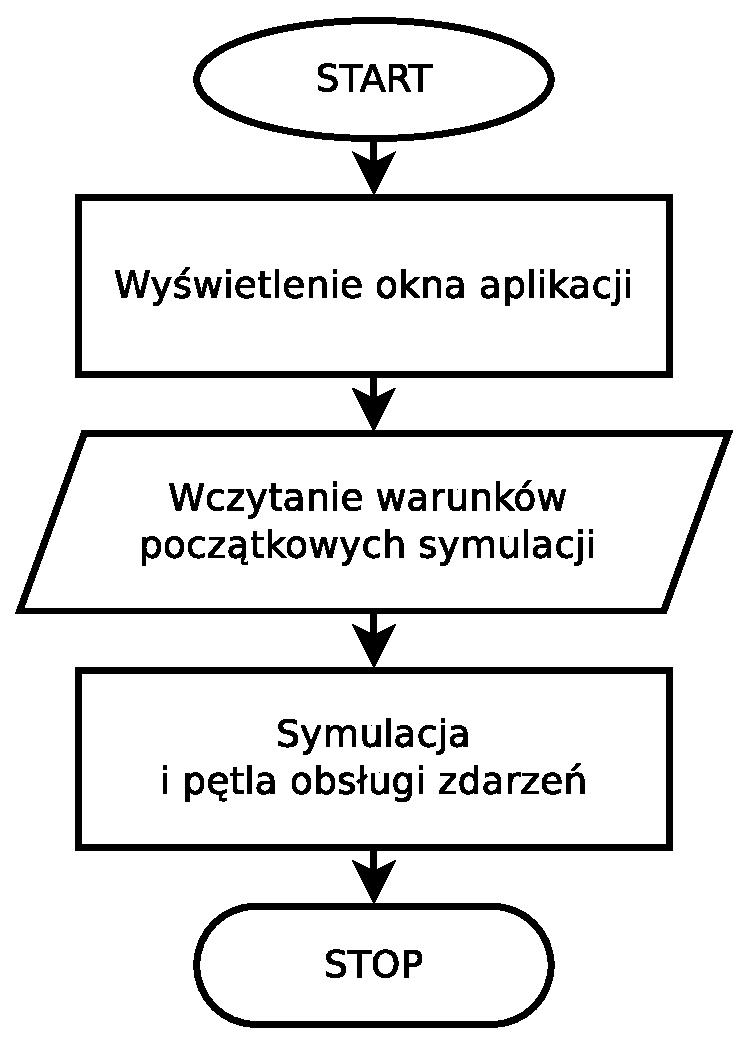
\includegraphics[scale=.4]{rysunki/diagram_przeplywu_sterowania}
 \end{center}
 \caption{Diagram przepływu sterowania}
 \label{fig:diagram_przeplywu_gui} 
\end{figure}   
%\bibliographystyle{abbrv}
%\nocite{*}
%\bibliography{bibliografia}

\end{document}

